\section{Processi Organizzativi}
\label{organizzativi}

% ruoli di progetto, gestione degli incontri, gestione degli strumenti di coordinamento e di versionamento, gestione dei rischi, gestione della formazione individuale

\subsection{Gestione dei processi}
    \subsubsection{Scopo}
    Qui lo scopo è la gestione delle attività e dei compiti per ogni altro processo.
    \subsubsection{Aspettative}
    L'organizzazione e la gestione dei compiti all'interno del gruppo di lavoro deve avvenire in modo sistematico, disciplinato e quantificabile così da favorire uno svolgimento dei lavori ordinato, che rispetti i tempi e che non sia vulnerabile a variazioni e problemi che si possono certamente riscontrare.
    \subsubsection{Descrizione}
    Il responsabile e l'amministratore si sono occupati della creazione e della configurazione di tutti gli ambienti necessari:
    \begin{itemize}
        \item account gmail;
        \item organizzazione GitHub;
        \item calendario condiviso su Google Calendar;
        \item workspace \href{https://slack.com/intl/en-it/about}{Slack};
        \item workspace Confluence con spazio dedicato ai verbali e spazio dedicato alle wiki;
        \item progetto Jira con board condivisa per l'organizzazione, gestione e tracciamento dei compiti.
    \end{itemize}
        \pparagraph{Jira}
        Come spiegato nella sezione \hyperref[jiraintegration]{Integrazione con Jira}, è stato configurato un processo automatico di collegamento fra commit su GitHub e task in Jira. Inoltre ad ogni azione, manuale o automatica, su Jira, viene generata una notifica nel canale dedicato di Slack.
        \pparagraph{workflow}
        \begin{figure}[H]
            \centering
            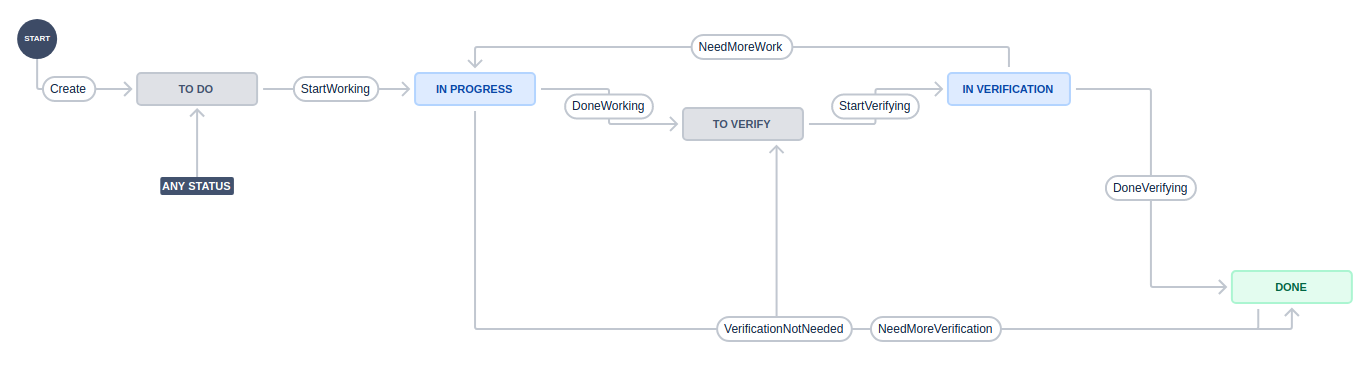
\includegraphics[scale=0.32]{res/images/jira_workflow.png}
            \caption{Diagramma degli stati e delle transizioni del workflow}
        \end{figure}
            Come si può vedere dall'immagine, il workflow di task e sottotask è stato configurato di modo che ci siano delle precise transizioni da uno stato all'altro e che solo quelle siano permesse. I nomi delle transizioni sulle frecce corrispondono ai comandi da usare nella sintassi degli smart commits. Maggiori dettagli si trovano nella wiki \textsc{Git, Github \& Jira}.

    \subsubsection{altre sottosezioni}
    ...
    \subsubsection{Strumenti}
    ...

\subsection{I ruoli di progetto}
    La suddivisione in ruoli è necessaria per favorire la parallelizzazione e distribuzione del lavoro e delle responsabilità.
    \subsubsection{Analista}
    Hai il compito specifico di comprendere il problema. Ha un ruolo attivo fin quando la comprensione non è adeguata. Adottando un modello incrementale, rimane più a lungo ed evolve. E auspicabile che ci siano più analisti per portare punti di vista diversi e sommare le conoscenze. Redige \textsc{Studio di Fattibilità} ed \textsc{Analisi dei Requisiti}.
    \subsubsection{Progettista}
    Traduce il problema in una possibile soluzione, descritta come architettura, divisa in parti per agevolare lo sviluppo individuale di queste. Dati i vincoli ha il compito di trovare una buona soluzione. Redige le specifiche tecniche e le definizioni del prodotto.
    \subsubsection{Verificatore}
    Agisce su ogni attività ed attua una verifica oggettiva, segnalando eventuali problemi secondo il \hyperref[label]{text}{processo rispettivo}.
    \subsubsection{Programmatore}
    Implementa in codice ciò che i progettisti hanno definito come design. Un'adeguata divisione dei compiti tra diversi programmatori consente un alto parallelismo, ideale per avanzare rapidamente. Deve svolgere compiti piccoli, che siano facilmente verificabili.
    \subsubsection{Responsabile}
    Gestisce il controllo sul progetto e tramite un cruscotto di controllo aggiorna, revisiona ed adatta lo svolgimento dei lavori. Elabora piani e scadenze, assegna compiti, approva documenti, gestisce i problemi, redige l'\textsc{Organigramma} ed il \textsc{Piano di Progetto} ed approva l'offerta prima di sottoporla al committente.
    \subsubsection{Amministratore}
    Ha in carico la definizione, modifica ed agevolazione del way of working. È un percorso in logica JiT procede per incrementi. È responsabile dell'efficacia e dell'efficienza nell'ambiente di lavoro, gestisce la documentazione, organizza il glossario, collabora alla redazione del \textsc{Piano di Progetto} e redige le \textsc{Norme di Progetto}.

\subsection{Infrastruttura} %todo
    \subsubsection{Scopo}
    Lo scopo del processo di ...
    \subsubsection{Aspettative}
    ...
    \subsubsection{Descrizione}
    ...
    \subsubsection{altre sottosezioni}
    ...
    \subsubsection{Strumenti}
    ...

\subsection{Miglioramento} %todo
    \subsubsection{Scopo}
    Lo scopo del processo di ...
    \subsubsection{Aspettative}
    ...
    \subsubsection{Descrizione}
    ...
    \subsubsection{altre sottosezioni}
    ...
    \subsubsection{Strumenti}
    ...

\subsection{Formazione} %todo
    \subsubsection{Scopo}
    Lo scopo del processo di ...
    \subsubsection{Aspettative}
    ...
    \subsubsection{Descrizione}
    ...
    \subsubsection{altre sottosezioni}
    ...
    \subsubsection{Strumenti}
    ...

\begin{comment}
\subsection{Comunicazione}
\subsubsection{Scopo}
Lo scopo del processo di ...

\subsection{Riunioni}
\subsubsection{Scopo}
Lo scopo del processo di ...

\subsection{Ruoli di Progetto}
\subsubsection{Scopo}
Lo scopo del processo di ...

\subsection{Ambiente di Lavoro}
\subsubsection{Scopo}
Lo scopo del processo di ...
\end{comment}